\chapter{Implementation details}
\label{ch:implementation_details}

This chapter aims to provide some insight into the technicalities in our development process, and to highlight the issues that we had to solve in order to get the final results. 

\section{\Matlab Processing}

Once we had acquired motion capture data of the actor's performance, we used \Matlab for the majority of the post-processing work before rendering the final output animation in \Maya using our own C++ plugins. All the stereo geometry processing was done in \Matlab, namely calibration of the stereo camera system, estimating the projection matrices and epipolar geometry, rectifying the image sequences, detecting and tracking the face markers, and finally computing the sparse 3D reconstructions of the facial expressions in each frame. Results from the tracking process, such as the tracking of the pupil movements and rigid head motion estimation, was output as a text file and read into C++ so as to be applied to the Maya model using the \Maya pugin. The solve for blendshape weights was also carried out in \Matlab, and the final weights were exported as a text file which could then be read into C++. 

\section{\Maya Plugin}
\label{sec:maya_plugin}

We used blendshape rigs for \Maya that are provided free by \cite{FaceWareRigsWeb}. The first task was to reset the paths of the texture files for all the materials in the Hypershade window in \Maya.
The next step was to write a plugin to load the weights from a text file exported from Matlab, and set keyframes for each of the blendshapes - to do this our plugin created a new \Maya command that could be easily executed. 
The work flow for writing the code was to first perform the action in \Maya manually if possible, see which MEL commands were executed, then implement them in the C++ plugin, and if possible rewrite them as pure C++ code instead of MEL commands.
Our code complies with \Maya's undo command policy, which means using the \emph{DagModifier} class or including extra code to undo the actions.
Nevertheless, in the final stages of the implementation, it was faster to reload the scene than to undo the command.

The text file format we use for the weights is one blendshape weight value per line in the order of the sequence of frames, as shown in Figure~\ref{fig:file_format}, where $N$ is the number of weights and $F$ is the number of frames.

\begin{figure}[htbp!]
\centering
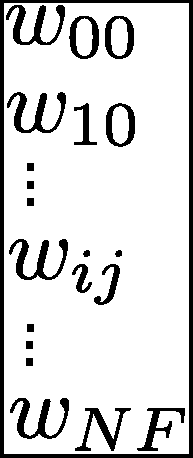
\includegraphics[width=0.1\textwidth]{img/file_format}
	\caption{The text file format used to store the blendshape weights for a given image sequence - used for exporting from \Matlab and importing into \Maya.}
	\label{fig:file_format}
\end{figure}

After reading in the weights from the text file, the connections between the blendshape object weights and their outputs have to be broken. This is done in order to be able to set the keyframes and update the blendshape values, otherwise the MEL command setKeyframe would not work. An extract of the code is shown in Listing~\ref{lst:set_weights}.
A minor point to highlight in this section is that the blendshape weights can be accessed using the following command, \textit{``shapesBS.weight[i]"}, however to break the connections the blendshape name in \Maya is needed.
To obtain a list with all the blendshape names the following command can be used, \textit{``listAttr -m shapesBS.w"}.
The weights will be listed in alphabetical order, yet the indices do not strictly follow the same order. 

\begin{lstlisting}[caption = Breaking the weights connections and setting keyframes., label = lst:set_weights, frame=single]

// Break connections.
for (unsigned int i = 0; i < (unsigned int)(numWeights); i++){
		cmd = "disconnectAttr shapesBS_";
		cmd = cmd + names[i];
		cmd = cmd + ".output shapesBS.";
		cmd = cmd + names[i];
		dgMod.commandToExecute(cmd);
}

// Set key frames
for (unsigned int j = 0; j < weights.at(i).size(); j++){
		cmd = "setAttr shapesBS.weight[";
		cmd = cmd + j;
		cmd = cmd + "] ";
		cmd = cmd + weights.at(i).at(j);
		dgMod.commandToExecute(cmd);
		
		cmd = "setKeyframe { \"shapesBS.w[";
		cmd = cmd + j;
		cmd = cmd + "]\" }";
		dgMod.commandToExecute(cmd);
	}
}
\end{lstlisting}

Once the blendshape weights for all frames in the sequence were added, we noticed that the teeth and tongue of the Emily rig would not move.
Both meshes were actually regulated by the position of a control object in the scene, so the solution was to translate the control object by a factor of the mean of all the blendshape weights involved in the control of the mouth, as shown in Listing~\ref{lst:teeth_tonge_control}.
The lower teeth and tongue would be left hanging in mid air when the mouth opens if the blendshapes that control the mouth opening were activated together; this problem was fixed by lowering the position of both meshes.

\begin{lstlisting}[caption = Teeth and tongue control based on relevant weights., label = lst:teeth_tonge_control, frame=single]

cmd = "setAttr con_jaw_c.translateY ";
cmd += -3.2 * (weights.at(i).at(58) + weights.at(i).at(55)) + 1;
dgMod.commandToExecute(cmd);
cmd = "setKeyframe  \"con_jaw_c.translateY\"";
dgMod.commandToExecute(cmd);
\end{lstlisting}

In order to make the animation more life-like, we decided to incorporate the removed rigid head rotation and translation back into the final animation.
In order to achieve this, we saved the inverse rotation for each frame from the Procustes analysis that was performed in Section~\ref{sec:stabilising_head_movement} into a file with the same format as shown in Figure~\ref{fig:file_format}.
We then read the data into \Maya using the plugin, and applied the transformation for each frame; for the translation we did an equivalent procedure with a translation file.
Note that Matlab matrices are column-wise while \Maya matrices are row-wise, so we read them into Maya taking this into account.
The matrix multiplication order also plays an important role here, as shown in Equation~\ref{eq:rotation_translation_inv}, where to achieve the correct resulting head pose, we need to undo the translation first and rotate the result.

\begin{equation}
\mathbf{x}_{new} = \mathbf{R} \mathbf{x} + \mathbf{t} ~ \rightarrow  \mathbf{R}^{-1}(\mathbf{x}_{new} - \mathbf{t}) = \mathbf{x},
\label{eq:rotation_translation_inv}
\end{equation}

where $\mathbf{x}$ is the original 3D point, $\mathbf{x}_{new}$ is the transformed point as a result of the Procrustes alignment, $\mathbf{R}$ is the rotation matrix and $\mathbf{t}$ is a translation vector.
We implemented this transformation in \Maya using the ``xform -m" command, first applying the translation and then applying the inverse rotation with an extra parameter ``-r" so that the matrices get multiplied in the desired order.

Having eye movement is quite important to achieve realism in the facial animation, so for this purpose we tracked the 3D world coordinate positions of the actor's pupils in the input image sequence.
These positions were saved into separate files for each eye using the same file format shown in Figure~\ref{fig:file_format}.
The positions were loaded into \Maya and the eye control object was translated using the offsets with respect to the first frame, which was assumed to be looking straight forward.
With this first approach, each eye can move independently which can lead to unsatisfactory results when one eye goes slightly off track and the other eye remains looking in the correct direction. An initial solution to this problem was to move both eyes together using the mean offset for each frame, so that their line of slight would always be parallel. This gave much better looking results, but nevertheless, this would still introduce considerable error when one of the eyes winks - since the tracking becomes completely unreliable for the winking eye which in turn drags the other eye with it.
Our solution involves interpolating between the two offsets using variable factors.
The idea is to have both eyes moving together, start ignoring the offset for an eye if it goes off, while sustaining smooth movements.
The final offset $d_f$ will be computed as $d_f = \alpha d_l + \beta d_r$, where $\alpha$ and $\beta$ are the interpolation factors, $d_l$ and $d_r$ are the offsets for the left and right eye, respectively.
Figure~\ref{fig:eyes_interpolation} shows the $\alpha_x$ values along the $x$-direction, where $t$ is the change threshold and $l$ is the maximum offset limit.
Initially $\alpha_x$ is $0.5$, however if the offset goes beyond a threshold $t$, $\alpha$ will decrease linearly until it reaches the limit $l$.
The same criteria will be applied in the $y$-direction, and the value for that eye will be $\alpha = \min \left\lbrace \alpha_x, \alpha_y \right\rbrace$.
The $\beta$ factor will be computed as $\beta = 1 - \alpha$, however, if the right eye is the one surpassing the threshold $t$, then the whole process will be reversed. 
Additionally, if both eyes surpass the threshold $t$, $\alpha$ and $\beta$ will be $0.5$, this will allow the eyes to move together beyond the threshold if needed.

\begin{figure}[htbp!]
\centering
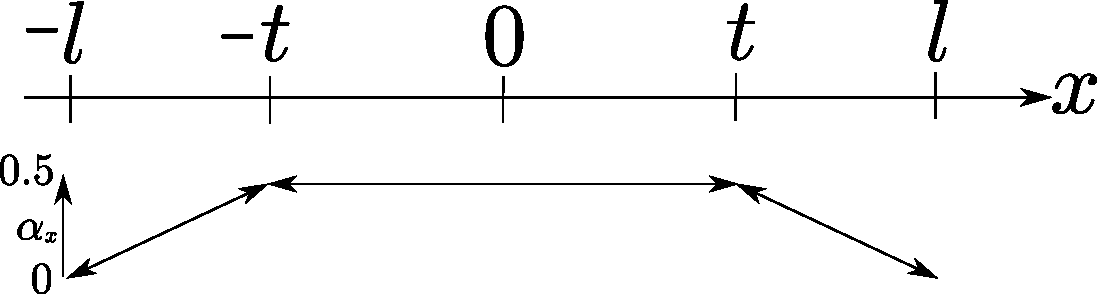
\includegraphics[width=0.8\textwidth]{img/eyes_interpolation}
	\caption{The offset interpolation for eye movements in \Maya. Here we are only considering the $x$-component of the pupil displacement, where 0 means the eye is looking straight forwards, and $l$ and $-l$ are the maximum and minimum pupil displacements respectively. }
	\label{fig:eyes_interpolation}
\end{figure}

Incorporating blinks was another important step towards attaining a more realistic animation.
Since the eyelids were not tracked in the recording session, the only option was to manually set the blinking times in \Maya.
To faithfully reproduce the blinking of the actor in the captured sequence the following information was manually added:
\begin{itemize}
\item Frame number marking when the eye:
	\begin{itemize}
	\item started closing;
	\item closed completely;
	\item started opening again;
	\item was fully open again;
	\end{itemize}
\item The blink magnitude (eyes fully closed, squinting, narrowing, etc);
\item The blink type (both eyes closed, only one eye).
\end{itemize}

As mentioned in Section~\ref{sec:estimation_w_actor_domain}, there is a mismatch between Emily's neutral face and the actor's neutral face.
In order to disguise this discrepancy as much as possible, a fixed constant was added to the blenshape weights controlling the smile, and we found that the best value for this constant was $0.35$.

%-----------------------------------------------------------------------------------------

\section{Skin Rendering}

Initially for all the Image Analogies work we used an implementation based on~\cite{ImAnSingleThreadWeb}.
This library was quite slow and it would not give results as good as the ones shown in the original paper.
We then moved to a parallel CUDA implementation~\cite{ImAnCudaWeb}; with this code the results were inconsistent, dependent on the number of threads, and exhibited erroneous pixel values, as shown in Figure~\ref{fig:cuda_error}.
The original code for Image Analogies has not been maintained since 2001, a patched version of the library, along with instruction on how to compile and run the code are provided alongside this report.

\begin{figure}[htbp!]
\centering
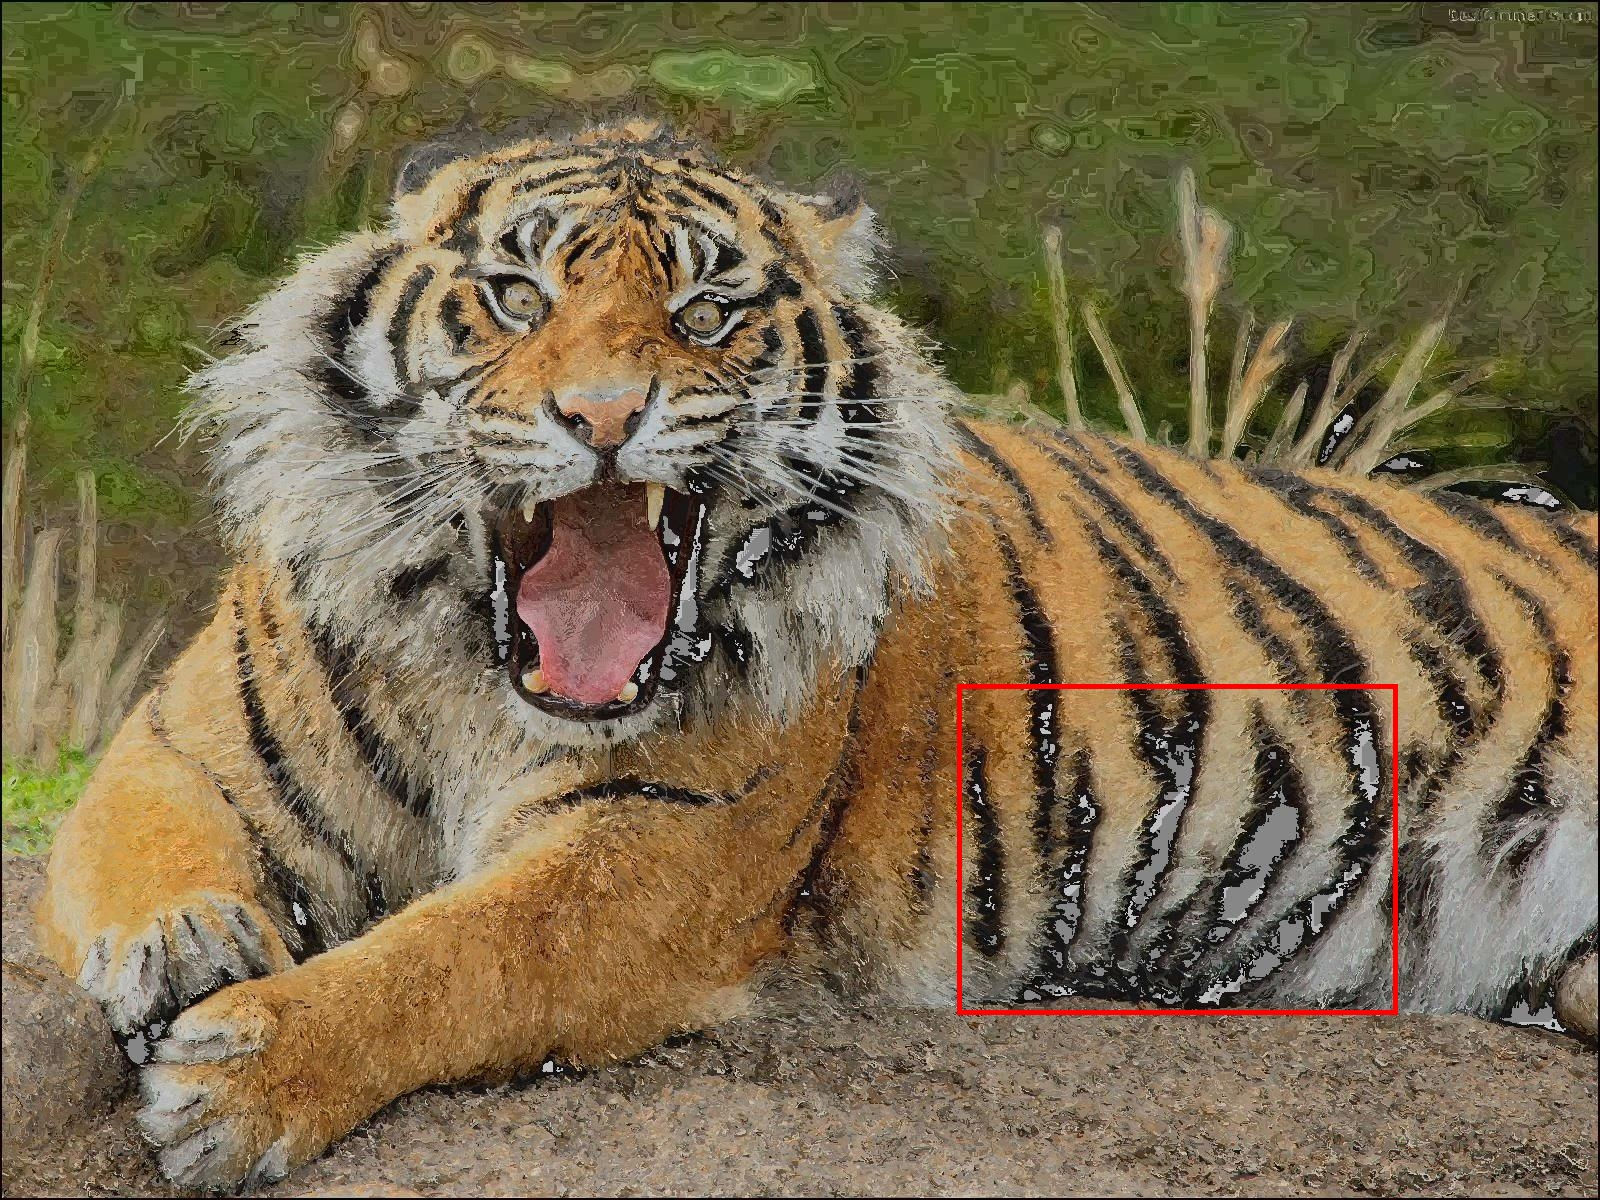
\includegraphics[width=0.5\textwidth]{img/cuda_error}
	\caption{Result for the CUDA Image Analogies implementation, erroneous values are highlighted in the red square, image taken from~\cite{ImAnCudaWeb}.}
	\label{fig:cuda_error}
\end{figure}

There are two important problems when using Image Analogies filter for adding detail to textures.
The first one arises due to the difference in colour distributions between the inputs.
For our data, there is a mismatch between images $\left\lbrace A, A' \right\rbrace$ and $B$, which was caused by divergent lighting conditions in the capture studio.
Since we have the prior knowledge that the images should represent the same areas on the face, we applied colour correction techniques to match the images.
The second issue derives from the local texture patch growth that the algorithm uses to replicate coherent patches in the input images.
If the kernel sizes does not match the features that we want to preserve in the example images, unconnected patches will be produced.
Moreover, this problem will be exacerbated with the face segmentation approach that was presented in Section~\ref{sec:metho_skin_rendering}.
In Figure~\ref{fig:skin_patch_error}, the top half of the image shows an example of such kernel size error, and the seam between the two areas is quite evident due to the patch segmentation.

\begin{figure}[htbp!]
\centering
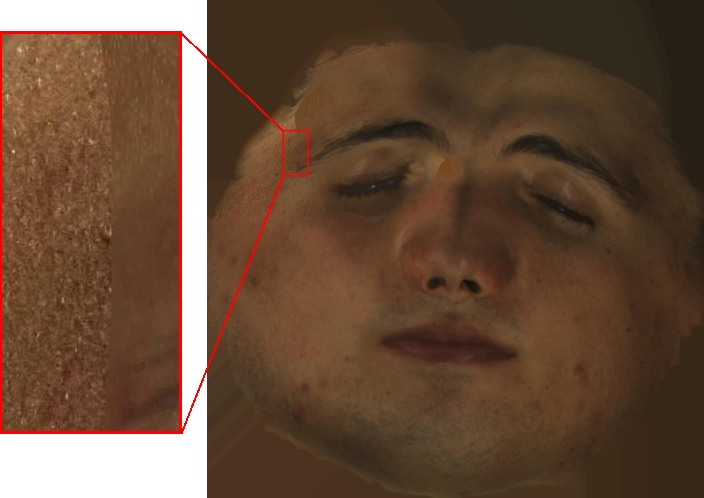
\includegraphics[width=0.6\textwidth]{img/skin_patch_error}
	\caption{Erroneously generated skin texture.}
	\label{fig:skin_patch_error}
\end{figure}

Normal map synthesis also required some pre- and post-processing steps for the pipeline to work.
The ground truth normal maps that we use as $\left\lbrace A, A' \right\rbrace$ were taken from Graham \textit{et al}.\cite{Graham2013}.
This data was encoded in the EXR format~\cite{EXRWeb}, which was not supported by the code we were using.
Each EXR image was converted to two PNG images, one encoding the positive values of the original data and the other encoding the negative ones.
The Image Analogies filter was run separately for each of them, and the results were recombined again into an EXR image.

To generate the results with the image super-resolution technique from Jianchao \textit{et al}.~\cite{Jianchao2010}, we made use of the image dictionaries provided by the authors.
In order to increase the quality and efficiency of the computation, the texture was divided into the segments introduced in Section~\ref{sec:metho_skin_rendering}.
Dividing the face into segments exploits more efficiency due to the nowadays more common multi-core CPU architectures, as we can run the algorithm for each patch independently.

